\documentclass{article}
\usepackage[a4paper]{geometry}
\usepackage[utf8]{inputenc}
\usepackage[utf8]{vietnam}
\usepackage{indentfirst}
\usepackage{graphicx}
\usepackage{hyperref}
\usepackage{url}
\usepackage{amsmath}
\usepackage[maxnames=4,backend=biber]{biblatex}

\graphicspath{ {images/} }
\addbibresource{faster-rcnn.bib}
\geometry{top=0.7in,bottom=0.7in}

\begin{document}


\title{Faster R-CNN: Towards Real-Time Object Detection with Region Proposal Networks}
\date{}
\author{Shaoqing Ren, Kaiming He, Ross Girshick, Jian Sun}

\begin{center}
	\Large{\textbf{Report}} \\
\end{center}

{\let\newpage\relax\maketitle }


\begin{flushright}
	\textbf{\textit{Students:} }\\
	Phạm Nguyễn Hoàng \\
	Trần Văn Liên \\
	Nguyễn Phạm Thiện Dũng \\
\end{flushright}

\section{Problem}

Object detection is a computer technology related to computer vision and image processing. The task of object detection is to detect instances of objects in certain classes such as humans, cars or animals \cite{wiki/object-detection}. Object detection has many applications and are widely used in many industries nowadays.

Input of the problem is the images which contain some objects to detect. Output is the labels of those objects and the bounding boxes for each object.

\begin{center}
	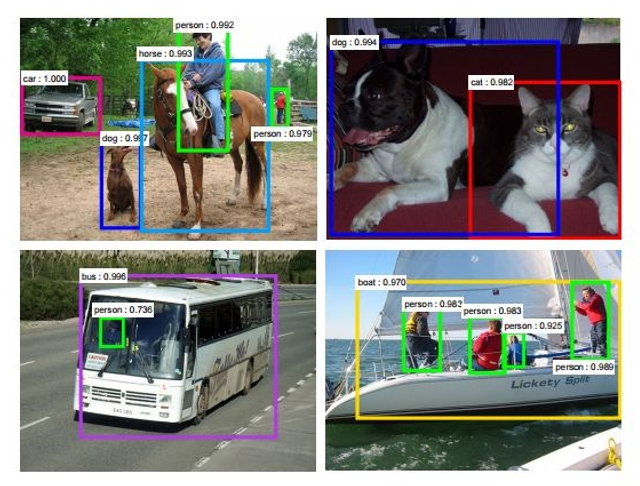
\includegraphics[scale=0.5]{object_detection}
\end{center}

\section{R-CNN}

R-CNN or Slow R-CNN is the first architecture in the R-CNN serie. We review R-CNN shortly in order to focus on Fast R-CNN and Faster R-CNN. The architecture of R-CNN is created from region proposals and CNNs \cite{arxiv/rcnn}.

\begin{center}
	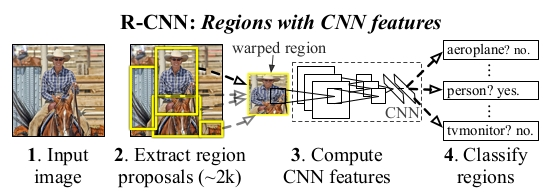
\includegraphics[scale=0.5]{rcnn}
\end{center}

R-CNN \textbf{region proposals} is selective search. A feature vector is extracted from each region proposal by a CNN. 

In test time, the selective search extract about 2000 region proposals per image. For each class, R-CNN extracts feature vector using a SVM which is trained for that class. After that, a greedy non-maximum suppression is applied to reject a region if it has an intersection-over-union (IoU) overlap with a higher scoring selected region than a learned threshold \cite{arxiv/rcnn}.

\noindent \textbf{R-CNN is trained using the following steps \cite{slides/rcnn-serie}:}
\begin{enumerate}
	\item Pre-train a convolutional neural network for ImageNet classification.
	\item Fine-tune the model from step 1 for object detection (using softmax classifier + log loss).
	\item Cache those feature vectors from step 2 to disk.
	\item Train linear SVMs on those feature vectors from step 3 (hinge loss).
	\item Train bounding box regressors on those feature vectors from step 3 (squared loss).
\end{enumerate}

\begin{center}
	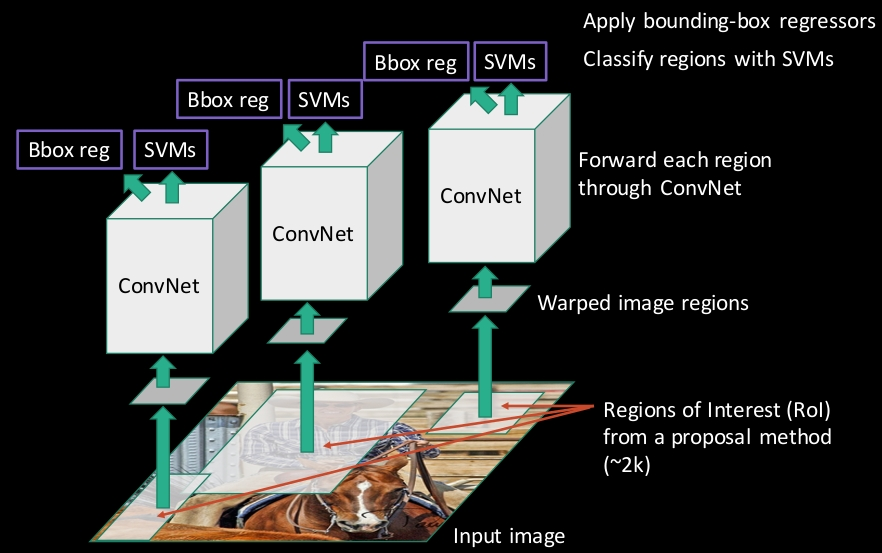
\includegraphics[scale=0.4]{rcnn_detail}
\end{center}

Each region proposal is processed through a convolution neural network and then classified by a SVM. This is considered as one of the reason that make R-CNN slow and inferior to Fast R-CNN.

\noindent \textbf{R-CNN has some disadvantages \cite{arxiv/fast-rcnn,slides/fast-rcnn}:}
\begin{enumerate}
	\item There are a lot of training procedures:
	\begin{itemize}
		\item Fine-tune the network with softmax classifier.
		\item Train linear SVMs for the features from the previous convolution neural network.
		\item Train bounding box regressors.
	\end{itemize}
	\item Training is very slow and takes a lot of disk space.
	\item Detection is slow (47s per image with VGG16).
\end{enumerate}

\section{SPPnet}

\textbf{Spatial Pyramid Pooling Net} (SPPnet) fixes the previous drawback of R-CNN. R-CNN has to forward each region proposal to a separate CNN. SPPnet makes testing time faster by computing a convolutional feature map for the entire image and classify each object proposal using this feature map. Therefore, we only need to forward this feature map to only a single CNN.

\begin{center}
	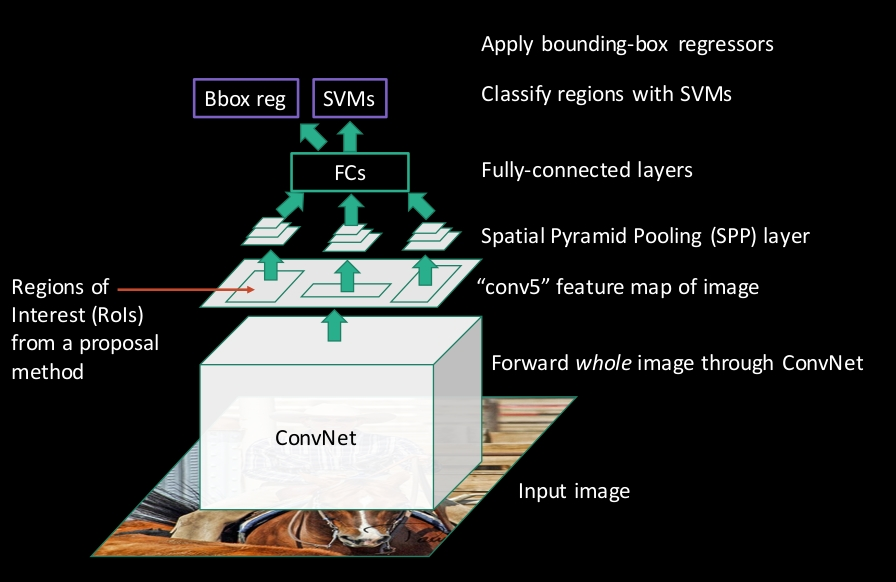
\includegraphics[scale=0.4]{sppnet_detail}
\end{center}

SPPNet also introduce \textbf{spatial pyramid pooling} layer which remove teh fixed-size constraint of the network. A SPP layer is added on top of the last convolutional layer to pool the features and generate fixed-length output \cite{arxiv/sppnet}.

\begin{center}
	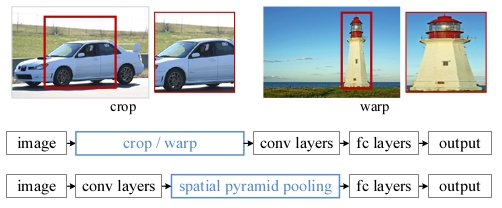
\includegraphics[scale=0.5]{sppnet}
\end{center}

\noindent \textbf{SPPnet is trained} by these following steps with 2 slightly different steps when training R-CNN \cite{slides/rcnn-serie}:
\begin{enumerate}
	\item Pre-train a convolutional neural network for ImageNet classification.
	\item \textbf{Cache SPP features to disk using the model from step 1.}
	\item \textbf{Train a new model by using the model from step 1 and fine-tune a 3-layer network from the features in step 2 (log loss).}
	\item Cache those feature vectors from step 3 to disk.
	\item Train linear SVMs on those feature vectors from step 3 (hinge loss).
	\item Train bounding box regressors on those feature vectors from step 3 (squared loss).
\end{enumerate}

The detail implementation of SPPnet can be see in \cite{arxiv/sppnet}. SPPnet is a big improvement for R-CNN and got an amazing result and beat a lot of opponents at that time.

However, SPPnet is unable to update weights below the spatial pyramid pooling layer. Back-propagation through SPP layer is inefficient when each training sample comes from a different image. each RoI may have a very large field (the size is usually approximately the same as the entire image). Therefore, the training inputs are large and the layer has to process a lot of data \cite{arxiv/faster-rcnn}.

\section{Fast R-CNN}

Fast R-CNN is an improvement to R-CNN and SPPnet in object classification. Fast R-CNN is 9 times faster than R-CNN and 3 times faster SPPnet. The detection network processes images in 0.3s (excluding object proposal time) and get a mAP of 66\% (R-CNN has a mAP of 62\%) \cite{arxiv/fast-rcnn}.

R-CNN and SPPnet have certain drawbacks which are stated in previous sections.
\begin{itemize}
	\item R-CNN is slow because it has to perform a ConvNet forward for each object proposal \cite{arxiv/fast-rcnn}.
	\item SPPnet fixes this drawback of R-CNN by computing a convolutional feature map for the entire image and classify each object proposal using this feature map. The training and testing speed are much faster than R-CNN. However, SPPnet has the following disadvantages:
	\begin{itemize}
		\item There are also a lot of training procedures.
		\item Training also takes lots of disk space.
		\item Fine-tuning algorithm cannot update the convolutional layers that precede the spatial pyramid pooling.
	\end{itemize}
\end{itemize}

\noindent \textbf{Fast R-CNN has the following advantages over these 2 architectures:}
\begin{enumerate}
	\item Higher detection quality.
	\item Faster training and testing time.
	\item Training can update all network layers.
	\item No disk storage is required.
\end{enumerate}

\noindent \textbf{Fast R-CNN architecture contains 4 steps}:
\begin{enumerate}
	\item Input is an image and a set of object proposals (output from \textbf{Selective Search}).
	\item The image is forwarded through some convolutional and max pooling layers to produce a feature map.
	\item A region of interest (RoI) pooling layer extracts a fixed-length feature vector from the feature map for each object proposal.
	\item Each feature vector is fed into some fully connected layers and finally 2 different layers:
	\begin{itemize}
		\item	One layer produces the sofmax probability that estimates over $K$ object classes and a background class.
		\item	One Layer gives the bounding boxes for each of $K$ object classes (each bounding box contains 4 numbers).
	\end{itemize}
\end{enumerate}

\begin{center}
	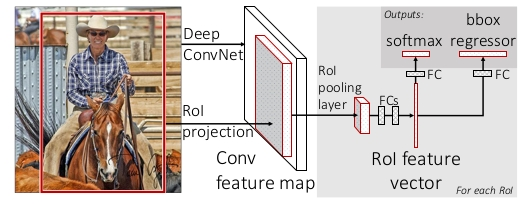
\includegraphics[scale=0.5]{fast_rcnn}
\end{center}

\textbf{The RoI pooling layer} use max pooling to convert any feature into a smaller feature map with a fixed size $H \times W$ (usually $7 \times 7$).  Each RoI is a rectangular window $(r, c, h, w)$ with the top-left corner $(r, c)$, the height $h$ and the width $w$.

\begin{center}
	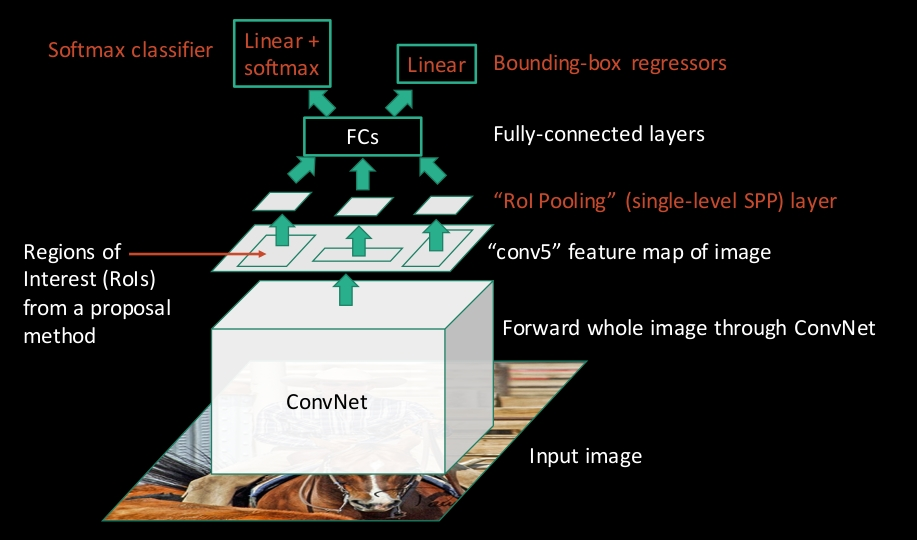
\includegraphics[scale=0.3]{fast_rcnn_detail}
\end{center}

RoI max pooling layer divides the $h \times w$ window into $H \times W$ sub-windows with approximate size $\dfrac{h}{H} \times \dfrac{w}{W}$ and max pools each sub-window to get the feature vector. 

Fast R-CNN, mini-batches for stochastic gradient descent are sampled hierarchically by sampling $N$ images and then sampling $\dfrac{R}{N}$ regions of interest (RoI) from each images. Normally $N = 2$ and $R = 128$. Fast R-CNN uses a streamlined training process with one fine-tuning stage that optimizes a softmax classifier and bounding box regressor simultaneously rather than different stages \cite{arxiv/fast-rcnn}.

\noindent \textbf{Fast R-CNN has 2 output layers:}
\begin{enumerate}
	\item  One layer outputs the probability distribution $p = (p_0,...,p_K)$ over $K + 1$ classes ($K$ classes and the background class).
	\item  One layer outputs the bounding boxes for $K$ classes $t^k = (t^k_x, t^k_y, t^k_w, t^k_h)$
\end{enumerate}

Each RoI is labeled with a ground truth class $u$ and a ground-truth bounding box regression target $v$. We have the following multi-task loss:
$$L(p, u, t_u, v) = L_{cls}(p, u) + \lambda [u \ge 1 ] L_{loc}(t^u, v)  $$

$L_{cls}(p, u) = -\log p_u$ is the log loss for the true class $u$. \\
$[u \ge 1] = 1$ when $u \ge 1$ and $0$ otherwise. \\
$L_{loc}$ is defined over the bounding-box regression target for class $u$ with $v = (v_x, v_y, v_w, v_h)$ and the predicted bounding box $t^u = (t^u_x, t^u_y, t^u_w, t^u_h)$.
$$L_{loc}(t^u, v) = \sum_{i \in \{x, y, w, h \}} smooth_{L_1}(t^u_i - v_i) $$
with 
$$smooth_{L_1}(x) = \begin{cases} 
   0.5x^2 & \text{if} |x| < 0 \\
   |x| - 0.5  & \text{otherwise}
  \end{cases}$$

\textbf{The mini-batches} are sampled with 64 RoIs from each image. 25\% of the RoIs are from object proposals that have the intersection over union (IoU) overlap with a ground truth bounding box of at least 0.5. The remaining RoIs are sampled from object proposals that have a maximum IoU with ground truth in the interval [0.1, 0.5).

For the \textbf{detection} phase:
\begin{enumerate}
	\item Fast R-CNN take an image as input and a list of $R$ object proposals.
	\item For each RoI $r$, the foward pass outputs a probability distribution $p$ and a set of predicted bounding box for $r$.
	\item Assign a detection confidence to $r$ for each object class $k$ using the estimated probability.
	\item Perform non-maxiumum supression independently for each class.
\end{enumerate}

The results are outstanding for Fast R-CNN \cite{slides/fast-rcnn}.

\begin{center}
	\begin{tabular}{| c | c | c | c |}
		\hline
		 & \textbf{Fast R-CNN} & \textbf{R-CNN}	& \textbf{SPPnet} \\
		\hline
		Training time & 9.5h & 84h & 25h \\
		Testing time / image & 0.32s & 47s & 2.3s  \\
		mAP & 66.9\% & 66.0\% & 63.1\% \\
		\hline
	\end{tabular}
\end{center}

\section{Faster R-CNN }

Faster R-CNN includes 2 modules:
\begin{enumerate}
	\item The first module is a deep fully convolutional network proposed regions.
	\item The second one is a Fast R-CNN detector which uses the proposed regions from the previous module.
\end{enumerate}

The entire system is a single and unified network for object detection. The Region Proposal Network gives the Fast R-CNN modules the regions to find the objects \cite{arxiv/faster-rcnn}. 

\begin{center}
	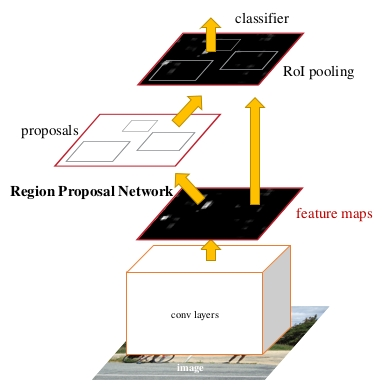
\includegraphics[scale=0.5]{faster_rcnn}
\end{center}

Here is the detailed structure of Faster R-CNN \cite{slides/faster-rcnn}.

\begin{center}
	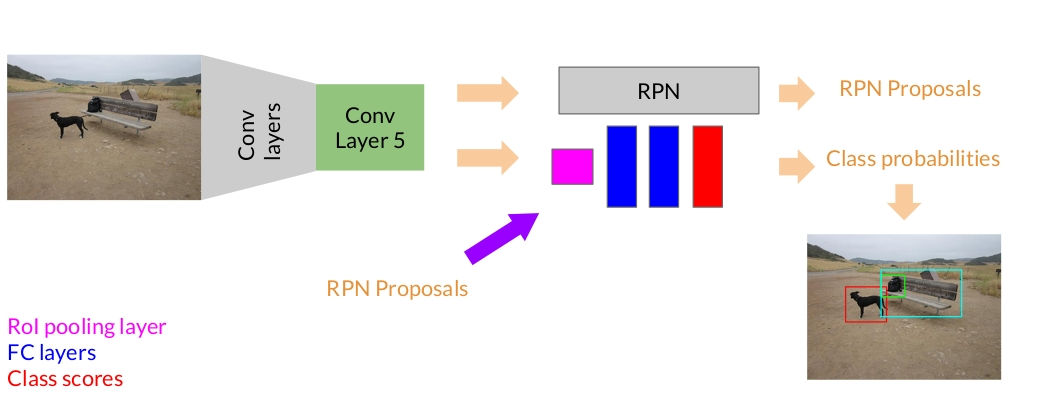
\includegraphics[scale=0.3]{faster_rcnn_detail}
\end{center}

A Region Proposal Network takes:
\begin{enumerate}
	\item \textbf{Input:} An image (any size)
	\item \textbf{Output: } A set of rectangular object proposals with objectness score. In the paper \cite{arxiv/faster-rcnn}, the authors tested 2 architectures: ZF Net \cite{arxiv/zfnet} and VGG-16 \cite{arxiv/vgg16}.
\end{enumerate}

In order to generate region proposals, a small network is slided over the convolutional feature map output by the last shared convolutional layer. This feature map is fed into 2 connected layers - a box-regression layer \textit{(reg)} and a box-classification layer \textit{(cls)}.

\begin{center}
	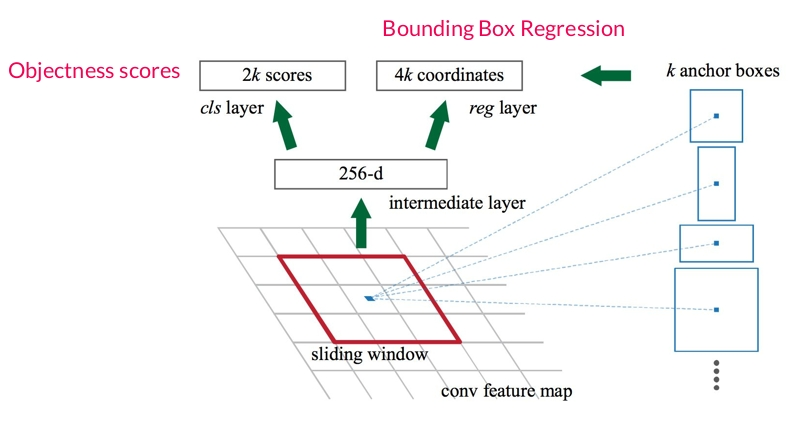
\includegraphics[scale=0.5]{faster_rcnn_rpn}
\end{center}

At each sliding location, the network simultaneously predict multiple region proposals with the maximum possible proposals for each location is $k$. Therefore, the \textit{reg} layer will have $4k$ outputs which encodes the rectangular coordinate for $k$ bounding boxes and $2k$ scores which estimate the probability of object or not object for each proposal \cite{arxiv/faster-rcnn}. The $k$ proposals are called \textit{anchors}. Each anchor is centered at the sliding window and has different ratio. For example, if $k = 9$, we would have those anchors \cite{videos/faster-rcnn}.

\begin{center}
	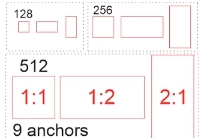
\includegraphics[scale=1.0]{faster_rcnn_anchors}
\end{center}

In order to train RPNs, a binary class label (being an object or not) is assigned to each anchor. A \textbf{positive label} is assigned when:
\begin{enumerate}
	\item	The anchor has the highest IoU (Intersection over Union) overlap with the ground truth box.
	\item	The anchor has an IoU overlap higher than 0.7 with any ground truth box.
\end{enumerate}

A \textbf{negative label} is assigned when the IoU ratio is lower than 0.3 for all ground truth boxes. 

The loss function for an image is defined:

$$L(\{p_i\},\{t_i\}) = \dfrac{1}{N_{cls}}\sum_{i} L_{cls}(p_i, p^*_i) + \lambda \dfrac{1}{N_{reg}} \sum_i p^*_i L_{reg}(t_i, t^*_i)$$

$i$ is the anchor. \\
$p_i$ is the predicted probability of being an object for anchor $i$. \\
$t_i$ is the coordinates of the predicted bounding box for anchor $i$. \\
$p^*_i$ is the ground truth object label, equals to 1 if the anchor is positive and 0 if the anchor is negative. \\
$t^*_i$ is the ground truth bounding box. \\
$L_{cls}$ is the log loss over 2 classes (object and not object). \\
$N_{cls}$ is the number of anchors in a mini-batch (set to 256 in general) \\
$N_{reg}$ is the number of anchor locations (about 2400). \\

For the bounding box regression, we calculate the paramaterers of the 4 coordinates:

$$t_x = \dfrac{x - x_a}{w_a}, t_y = \dfrac{y - y_a}{h_a}$$
$$t_w = \log \dfrac{w}{w_a}, t_h = \log \dfrac{h}{h_a}$$
$$t^*_x = \dfrac{x^* - x_a}{w_a}, t^*_y = \dfrac{y^* - y_a}{h_a}$$
$$t^*_w = \log \dfrac{w^*}{w_a}, t^*_h = \log \dfrac{h^*}{h_a}$$

where $x, y, w, h$ is the predicted box's center coordinates, width and height respectively. $x_a, y_a, w_a, h_a$ is for the anchor box and $x^*, y^*, w^*, h^*$ is for the ground truth box. The feature used for regression are of the same spatial size on the feature maps. $k$ bounding-box regressors are learned for each ratio and do not share weights \cite{arxiv/faster-rcnn}.

The RPN is trained by back propagation and stochastic gradient descent. Each mini-batch is selected from 256 random anchors of an image which contains 128 positive samples and 128 positive negative samples. If there are fewer than 128 positive samples, negative samples will be added. Weights are randomly initialized from Gaussian distribution ($\mu = 0, \sigma = 0.001$). The learning rate is 0.001 for the first 60,000 mini-batches and 0.0001 for the next 20,000 mini-batches when training on PASCAL VOC dataset \cite{arxiv/faster-rcnn}.

For the second phase (detection), Fast R-CNN is used.  However, a unified network compose of RPN and Fast R-CNN with shared convolutional layers are learned. There are 4 steps for training \cite{slides/faster-rcnn}:

\begin{enumerate}
	\item Train RPN initialized with an ImageNet pre-trained model.
	\begin{center}
		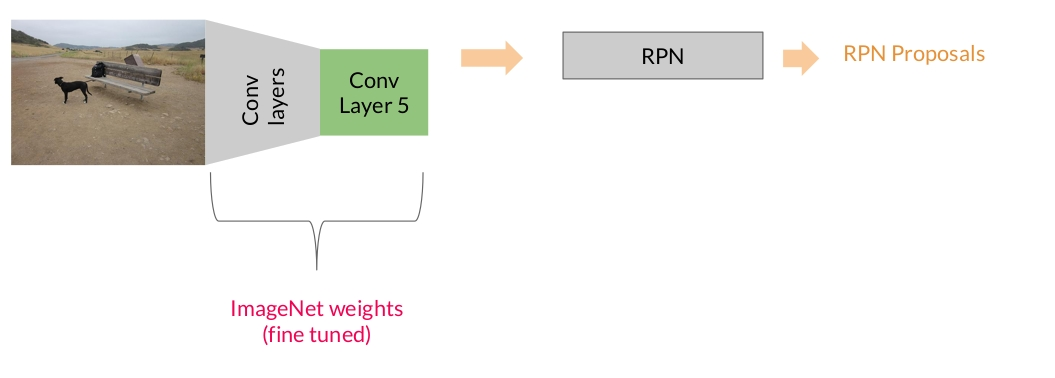
\includegraphics[scale=0.3]{faster_rcnn_step_1}
	\end{center}
	\item Train Fast R-CNN with learned RPN proposals
	\begin{center}
		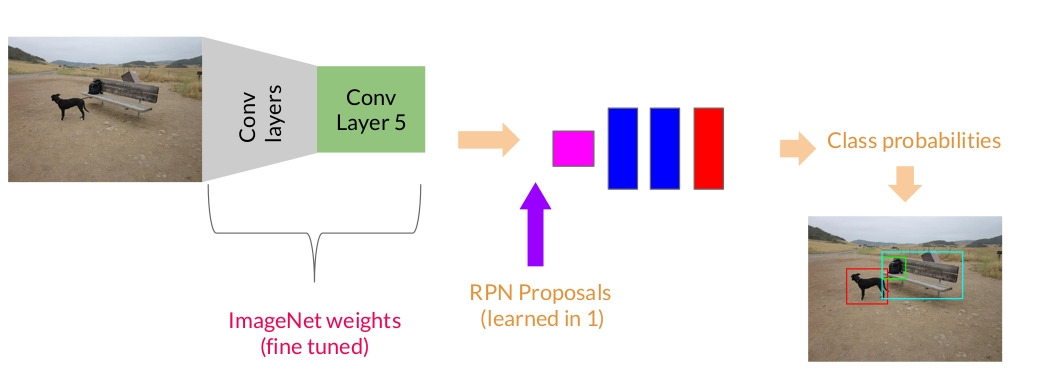
\includegraphics[scale=0.3]{faster_rcnn_step_2}
	\end{center}
	\item The model from step 2 is used to initialize RPN and re-train.
	\begin{center}
		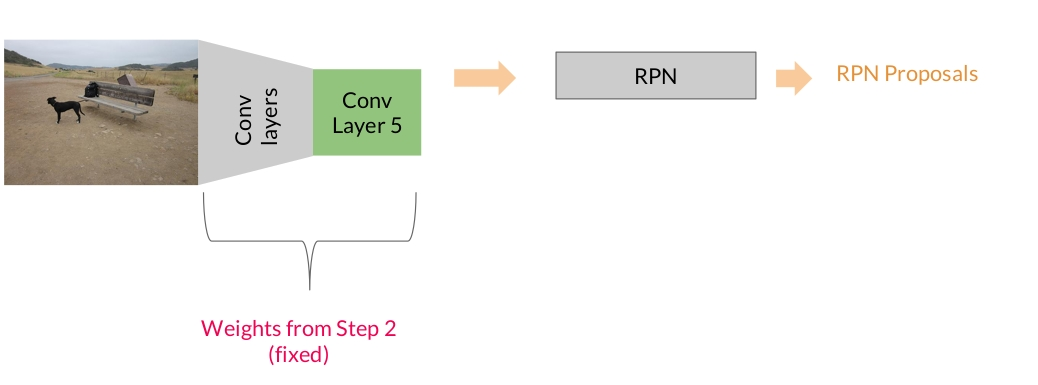
\includegraphics[scale=0.3]{faster_rcnn_step_3}
	\end{center}
	\item Fine tune the fully connected layer of Fast R-CNN using the shared convolutional layers as in step 3.
	\begin{center}
		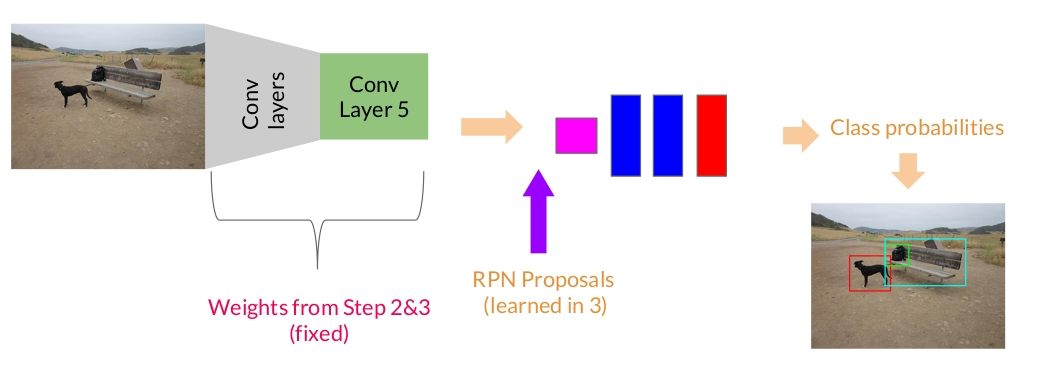
\includegraphics[scale=0.3]{faster_rcnn_step_4}
	\end{center}
\end{enumerate}

The results are much better in speed when comparing Faster R-CNN with R-CNN and Fast R-CNN. Here is the comparison of these 3 architectures on VOC 2007 \cite{videos/faster-rcnn}.
\begin{center}
	\begin{tabular}{| c | c | c | c |}
		\hline
		 & \textbf{R-CNN} & \textbf{Fast R-CNN}	& \textbf{Faster R-CNN} \\
		\hline
		Test time per image & 50s & 2s & 0.2s \\
		mAP & 66.0\% & 66.9\% & 66.9\%  \\
		\hline
	\end{tabular}
\end{center}

\section{Experimental Result}

The Python implementation of Faster R-CNN is hosted at \url{https://github.com/rbgirshick/py-faster-rcnn}. We have modified the original $demo.py$ file (used for object detection in still images) in order to detect people from a live camera feed. On a laptop computer with an NVIDIA 940MX graphics card and Core i5-6200U, detection takes approximately 0.6 seconds for each 640x480 frame. An image of the program running on Ubuntu is shown below. 

\begin{center}
	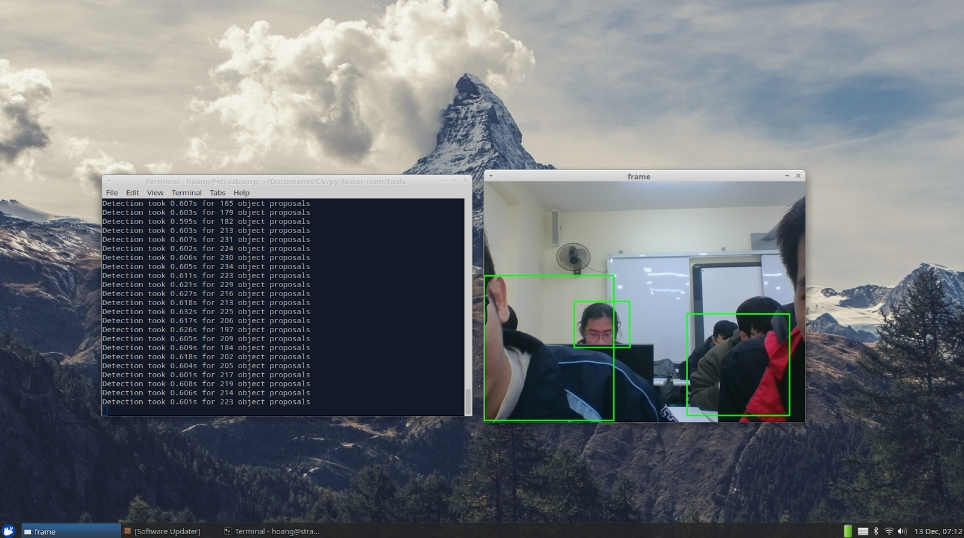
\includegraphics[scale=0.4]{faster_rcnn_result}
\end{center}

\clearpage
\printbibliography[title={References}]

\end{document}